        \documentclass{standalone}
        \usepackage{tikz}
        \usetikzlibrary{arrows}
        \usepackage{amsmath}
        \usepackage{amsfonts}
        \begin{document}
        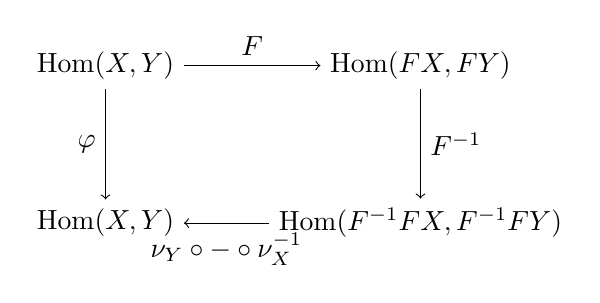
\begin{tikzpicture}

    \node at (0,0) (start) {$\operatorname{Hom}(X,Y)$};
    \node at (4,0) (F) {$\operatorname{Hom}(FX,FY)$};
    \node at (4,-2) (G) {$\operatorname{Hom}(F^{-1}FX,F^{-1}FY)$};
    \node at (0,-2) (end) {$\operatorname{Hom}(X,Y)$};
    \draw[->] (start) -- node[above] {$F$} (F);
    \draw[->] (F) -- node[right] {$F^{-1}$} (G);
    \draw[->] (G) -- node[below] {$\nu_Y \circ - \circ \nu^{-1}_X$} (end);
    \draw[->] (start) -- node[left] {$\varphi$} (end);
        \end{tikzpicture}
        \end{document}
